\documentclass[twoside,twocolumn]{ltjsarticle}
\usepackage{silence}
\WarningFilter{caption}{Unknown document}
\usepackage[top=20truemm,bottom=20truemm,left=15truemm,right=15truemm,headheight=20pt]{geometry}
\usepackage{fancyhdr,lastpage,abstract,listings,float,wrapfig,tabularx,multirow}
\usepackage{hyperref,graphics,graphicx,framed,subcaption}
\usepackage[symbol]{footmisc}
\usepackage{amsmath,amssymb}
\usepackage{tikz}
\usetikzlibrary{calc,arrows.meta,fit,positioning,math}
\newcolumntype{A}{>{\centering\bfseries}X}
\newcolumntype{B}{>{\centering\bfseries\arraybackslash}X}
\newcolumntype{C}{>{\centering\arraybackslash}X}
\newcolumntype{R}{>{\raggedright\arraybackslash}X}
\newcolumntype{L}{>{\raggedleft\arraybackslash}X}
\bibliographystyle{junsrt}
\hypersetup{
    colorlinks=true,
    citecolor=black,
    linkcolor=black,
    urlcolor=black
}
\fancypagestyle{report}{
    \fancyhf{}
    \fancyhead[RO,LE]{}
    \fancyfoot[RO,LE]{\thepage\ /\ \pageref{LastPage}}
    \pagenumbering{arabic}
    \renewcommand{\headrulewidth}{0mm}
}
\lstset{
    language = {Matlab},
    %backgroundcolor={\color[gray]{.90}},
    breaklines = true,
    breakindent = 10pt,
    basicstyle = \ttfamily\small,
    commentstyle = {\ttfamily \color[rgb]{0,0.45,0}},
    classoffset = 0,
    keywordstyle = {\bfseries \color{magenta}},
    stringstyle = {\ttfamily \color{blue}},
    frame = left,
    %他オプション:leftline,topline,bottomline,lines,single,shadowbox
    framesep = 5pt,
    numbers = none,
    stepnumber = 1,
    numberstyle = \small,
    tabsize = 4,
    captionpos = t,
    otherkeywords = {xticks, yticks, exportgraphics, imwrite, bitshift, uint8, double}
}
\renewcommand{\figurename}{図}
\renewcommand{\tablename}{表}
\renewcommand{\lstlistingname}{src.}
\renewcommand{\thefootnote}{\fnsymbol{footnote}}
\renewcommand{\contentsname}{目次}
\renewcommand{\listfigurename}{図目次}
\renewcommand{\listtablename}{表目次}
\renewcommand{\lstlistlistingname}{ソースコード}
\renewcommand{\thefigure}{\arabic{figure}}
\renewcommand{\thetable}{\arabic{table}}
\renewcommand{\theequation}{\arabic{equation}}
% \renewcommand{\thesubfigure}{(\alph{subfigure})}
\renewcommand{\labelenumi}{\textbf{\theenumi}.\ }
\renewcommand{\eqref}[1]{式(\ref{#1})}
\newcommand{\matlab}{\text{{\large M}ATLAB\raisebox{2mm}{\tiny\textregistered}}}
\newcommand{\mat}[2]{\(#1\)行\(#2\)列}
\newcommand{\figref}[1]{図\ref{#1}}
\newcommand{\tblref}[1]{表\ref{#1}}
\newcommand{\srcref}[1]{src.\ref{#1}}
\newcommand{\scall}[1]{課題\ (#1)\ のスクリプトは,}
\newcommand{\sref}[1]{\(\underset{\blacktriangleright\textrm{p.\pageref{#1}}}{\textrm{\srcref{#1}}}\)}
% \captionsetup[subfigure]{labelformat=simple}
\makeatletter
\@addtoreset{figure}{section}
\@addtoreset{table}{section}
\@addtoreset{lstlisting}{section}
\@addtoreset{footnote}{page}
\makeatother
\AtBeginDocument{
    \renewcommand{\thelstlisting}{\thesection-\arabic{lstlisting}}
}
\title{{\normalsize 情報学群実験第3C/3i 実験レポート 第3回}\\WEBページ上のカラーユニバーサルデザインに関する実験}
\author{1250373\hspace{1\zw}溝口 洸熙\thanks{高知工科大学 情報学群 情報セキュリティシステム研究室}\\Group 10}
\date{June 7th, 2023}
% paragraph command
\newcommand{\purpose}{実験の背景と目的}
\newcommand{\method}{実験の方法}
\newcommand{\result}{実験の結果}
\newcommand{\consideration}{考察}
\newcommand{\conclusion}{結論}
% 課題1
\newcommand{\kadaia}{画像の理解}
\newcommand{\kadaiaa}{カラーチャネル操作}
\newcommand{\kadaiab}{画像の量子化数変換}
\newcommand{\kadaiac}{階調反転}
\newcommand{\kadaiad}{閾値処理}
\newcommand{\kadaiae}{ヒストグラム}
\newcommand{\kadaiaf}{背景差分}
% 課題2
\newcommand{\kadaib}{画像のフィルタ処理}
\newcommand{\kadaiba}{テスト画像作成}
\newcommand{\kadaibb}{平滑化フィルタ・メディアンフィルタ}
\newcommand{\kadaibc}{微分フィルタ}
\newcommand{\kadaibd}{ラプラシアンフィルタ}
\newcommand{\kadaibe}{色空間変換}
% 課題3
\pagestyle{report}
\begin{document}
\twocolumn[
    \maketitle
    \thispagestyle{report}
    \renewcommand{\abstractname}{概要}
\begin{abstract}
    今回の実験では,眼球運動測定実験,行動実験,脳波測定実験をする.
    眼球運動では,顔画像の印象に関する判断についての眼球運動と,対象を自由に見るときの眼球運動を計測する.
    カスケード現象より選好する顔画像を選択する直前の視線の向き,またポスターに対する注視する箇所について明らかになった.
    行動実験では,多数ある妨害刺激中に目標刺激が有るか否かを判断し,刺激数と探索時間の関係を確認する.
    結果に対して回帰直線の傾きを求め,刺激の種類によって回帰直線が異なることが,統計的仮説検定を用いて明らかとなった.
    脳波測定実験では,BMI装置を用いて脳波を読み取り,指定したターゲット刺激が表示された脳波はそうでない場合の脳波に比べて電位の振れが大きいことが分かった.
\end{abstract}

]
\saythanks
\chapter{画像情報処理}
\section{\purpose}
\matlab を用いて,画像に対して,カラーチャネルの操作,量子化数変換,階調反転,閾値処理,画素値に対するヒストグラムを作成など,基本的な画像処理を行う.\par
また,HSV色空間上で肌色の抽出をする.HSV色空間の特徴として,人間が色を知覚する方法と類似していることが挙げられる.視覚障害者向けのアクセシビリティ向上に役立つ\cite[p.97\ -\ p.98]{画像処理}.
人間が色を知覚する方法と類似していることを踏まえて,HSV色空間を用いることで,画像の特徴を抽出しやすくなる.今回の実験では,自分の手の写真をRGB色空間からHSV色空間へ変換し,肌色領域を抽出する.抽出した肌色領域を白色,そのほかの部分を黒色にして出力する.出力した画像と,RGB色空間における肌色領域を抽出した場合の精度について考察する.\par
さらに,ノイズ画像に対して,ノイズ除去する.周囲画素値の平均値を中央の画素値にする平滑化フィルタと,周囲画素値の中央値を中央の画素値にするメディアンフィルタを,ノイズの雑音除去具合で比較する.\par
加えて,画像のエッジを検出するために,微分フィルタを適用する.今回適用する微分フィルタは,SobelフィルタとLaplacianフィルタである.両フィルタで抽出できるエッジの精度について考察する.\par
最後に,画像を2次元フーリエ変換し,パワースペクトルを出力する.出力したパワースペクトルに対して,高域通過フィルタを適用し,画像座標とパワースペクトル画像座標の関係と,パワースペクトル各値の意味を明らかにする.
\section{\method}
\paragraph{実験に用いる装置}このレポート内すべての実験にはMathWorks\raisebox{2mm}{\tiny\textregistered}社の\matlab を用いて,\tblref{tbl:実験環境}の環境下で実験する.
\begin{table}[H]
    \caption{実験環境}
    \label{tbl:実験環境}
    \begin{tabularx}{\columnwidth}{cR}
        \hline
        \multirow{2}{*}{実験機}   & MacBook Air 2022 (Apple社)   \\
                               & 型番:\texttt{MLY13J/A}        \\
        \hline
        \multirow{2}{*}{プロセッサ} & Apple Silicon M2            \\
                               & 8コアCPU,8コアGPU               \\
        メモリ                    & 8GB                         \\
        \hline
        Webブラウザ                & Safari\ バージョン16.5           \\
        \hline
        ImageJ                 & 1.53k\ Java 13.0.6 (64-bit) \\
        \hline
    \end{tabularx}
\end{table}
\paragraph{CSS}
CSSとは,
\section{\result}
\newcommand{\axisfig}[1]{
    \begin{tikzpicture}
        \node (fig){\includegraphics[width=.9\textwidth,keepaspectratio]{#1}};
        \node[left] at ($(fig.south west)!0.5!(fig.north west)+(0.2cm,0)$){\rotatebox{90}{\tiny \texttt{frequency}}};
        \node[below] at ($(fig.south west)!0.5!(fig.south east)+(0,0.2cm)$){\rotatebox{0}{\tiny \texttt{frequency}}};
    \end{tikzpicture}
    \vspace{-2em}
}
\begin{figure}[H]
    \centering
    \begin{minipage}[b]{.19\textwidth}
        \centering
        \includegraphics[keepaspectratio,width=\textwidth]{../../kut.jpg}
        \subcaption{元画像}
        \label{fig:元画像}
    \end{minipage}
    \begin{minipage}[b]{.19\textwidth}
        \centering
        \includegraphics[keepaspectratio,width=\textwidth]{../../Figures/05_11_r.png}
        \subcaption{赤チャネル}
    \end{minipage}
    \begin{minipage}[b]{.19\textwidth}
        \centering
        \includegraphics[keepaspectratio,width=\textwidth]{../../Figures/05_12_g.png}
        \subcaption{緑チャネル}
    \end{minipage}
    \begin{minipage}[b]{.19\textwidth}
        \centering
        \includegraphics[keepaspectratio,width=\textwidth]{../../Figures/05_13_b.png}
        \subcaption{青チャネル}
    \end{minipage}
    \begin{minipage}[b]{.19\textwidth}
        \centering
        \includegraphics[keepaspectratio,width=\textwidth]{../../Figures/05_14_change.png}
        \subcaption{赤青チャネル入れ替え}
    \end{minipage}
    \caption{\kadaiaa\ 実験結果}
    \begin{minipage}[b]{.23\textwidth}
        \centering
        \includegraphics[keepaspectratio,width=\textwidth]{../../Figures/05_21_gimg.png}
        \subcaption{量子化数\ 8Bit\footnotemark[1]}
    \end{minipage}
    \begin{minipage}[b]{.23\textwidth}
        \centering
        \includegraphics[keepaspectratio,width=\textwidth]{../../Figures/05_22_4bit.png}
        \subcaption{量子化数\ 4Bit}
    \end{minipage}
    \begin{minipage}[b]{.23\textwidth}
        \centering
        \includegraphics[keepaspectratio,width=\textwidth]{../../Figures/05_23_2bit.png}
        \subcaption{量子化数\ 2Bit}
    \end{minipage}
    \begin{minipage}[b]{.23\textwidth}
        \centering
        \includegraphics[keepaspectratio,width=\textwidth]{../../Figures/05_24_1bit.png}
        \subcaption{量子化数\ 1Bit}
    \end{minipage}
    \caption{\kadaiab\ 実験結果}
    \begin{minipage}[b]{.23\textwidth}
        \centering
        \includegraphics[keepaspectratio,width=\textwidth]{../../Figures/05_31_8.png}
        \subcaption{量子化数\ 8Bit}
    \end{minipage}
    \begin{minipage}[b]{.23\textwidth}
        \centering
        \includegraphics[keepaspectratio,width=\textwidth]{../../Figures/05_32_4.png}
        \subcaption{量子化数\ 4Bit}
    \end{minipage}
    \begin{minipage}[b]{.23\textwidth}
        \centering
        \includegraphics[keepaspectratio,width=\textwidth]{../../Figures/05_33_2.png}
        \subcaption{量子化数\ 2Bit}
    \end{minipage}
    \begin{minipage}[b]{.23\textwidth}
        \centering
        \includegraphics[keepaspectratio,width=\textwidth]{../../Figures/05_34_1.png}
        \subcaption{量子化数\ 1Bit}
    \end{minipage}
    \caption{\kadaiac\ 実験結果}
\end{figure}
\begin{figure}[H]
    \begin{minipage}[b]{.7\textwidth}
        \centering
        \begin{minipage}[b]{.3\textwidth}
            \centering
            \includegraphics[keepaspectratio,width=\textwidth]{../../Figures/05_41.png}
            \subcaption{閾値\ \(64\)}
        \end{minipage}
        \begin{minipage}[b]{.3\textwidth}
            \centering
            \includegraphics[keepaspectratio,width=\textwidth]{../../Figures/05_42.png}
            \subcaption{閾値\ \(128\)}
        \end{minipage}
        \begin{minipage}[b]{.3\textwidth}
            \centering
            \includegraphics[keepaspectratio,width=\textwidth]{../../Figures/05_43.png}
            \subcaption{閾値\ \(192\)}
        \end{minipage}
        \caption{\kadaiad\ 実験結果}
    \end{minipage}
    \begin{minipage}[b]{.25\textwidth}
        \centering
        \includegraphics[keepaspectratio,width=\textwidth]{../../Figures/05_50_graph.pdf}
        \caption{\kadaiae\ 実験結果}
    \end{minipage}
\end{figure}
\begin{figure}[H]
    \begin{minipage}[b]{.49\textwidth}
        \centering
        \begin{minipage}[b]{.3\textwidth}
            \centering
            \includegraphics[keepaspectratio,width=\textwidth]{../../05_UnderstandingImages/fig1_g.jpg}
            \subcaption{被写体と背景}
        \end{minipage}
        \begin{minipage}[b]{.3\textwidth}
            \centering
            \includegraphics[keepaspectratio,width=\textwidth]{../../05_UnderstandingImages/fig2_g.jpg}
            \subcaption{背景のみ}
        \end{minipage}
        \begin{minipage}[b]{.3\textwidth}
            \centering
            \includegraphics[keepaspectratio,width=\textwidth]{../../Figures/05_60.png}
            \subcaption{背景差分画像}
        \end{minipage}
        \caption{\kadaiaf\ 実験結果}
    \end{minipage}
    \nextfloat
    \begin{minipage}[b]{.49\textwidth}
        \centering
        \begin{minipage}[b]{.3\textwidth}
            \centering
            \includegraphics[keepaspectratio,width=\textwidth]{../../Figures/05_61.png}
            \subcaption{閾値\ \(32\)}
        \end{minipage}
        \begin{minipage}[b]{.3\textwidth}
            \centering
            \includegraphics[keepaspectratio,width=\textwidth]{../../Figures/05_62.png}
            \subcaption{閾値\ \(64\)}
        \end{minipage}
        \begin{minipage}[b]{.3\textwidth}
            \centering
            \includegraphics[keepaspectratio,width=\textwidth]{../../Figures/05_63.png}
            \subcaption{閾値\ \(128\)}
        \end{minipage}
        \caption{背景差分画像の閾値処理}
    \end{minipage}
\end{figure}
\footnotetext[1]{NTSC輝度信号のグレイスケール画像}
\begin{figure}[h]
    \centering
    \begin{minipage}[b]{.3\textwidth}
        \centering
        \includegraphics[keepaspectratio,width=\textwidth]{../../Figures/05_21_gimg.png}
        \subcaption{元画像}
    \end{minipage}
    \begin{minipage}[b]{.3\textwidth}
        \centering
        \includegraphics[keepaspectratio,width=\textwidth]{../../06_ImageFiltering/file_white-Gaussian-Noise.png}
        \subcaption{白色ガウス雑音(\wgnimg)}
    \end{minipage}
    \begin{minipage}[b]{.3\textwidth}
        \centering
        \includegraphics[keepaspectratio,width=\textwidth]{../../06_ImageFiltering/file_impluse-noise.png}
        \subcaption{インパルス雑音(\inimg)}
    \end{minipage}
    \caption{\kadaiaa\ 実験結果}
\end{figure}
\begin{figure}[H]
    \centering
    \begin{minipage}[b]{.49\textwidth}
        \begin{minipage}[b]{.49\textwidth}
            \includegraphics[keepaspectratio,width=\textwidth]{../../Figures/06_21_sf_img_wgn.png}
            \subcaption{\wgnimg}
        \end{minipage}
        \begin{minipage}[b]{.49\textwidth}
            \includegraphics[keepaspectratio,width=\textwidth]{../../Figures/06_22_sf_img_in.png}
            \subcaption{\inimg}
        \end{minipage}
        \caption{平滑化フィルタ}
    \end{minipage}
    \begin{minipage}[b]{.49\textwidth}
        \begin{minipage}[b]{.49\textwidth}
            \includegraphics[keepaspectratio,width=\textwidth]{../../Figures/06_23_mf_img_wgn.png}
            \subcaption{\wgnimg}
        \end{minipage}
        \begin{minipage}[b]{.49\textwidth}
            \includegraphics[keepaspectratio,width=\textwidth]{../../Figures/06_24_mf_img_in.png}
            \subcaption{\inimg}
        \end{minipage}
        \caption{メディアンフィルタ}
    \end{minipage}
\end{figure}
\begin{figure}[H]
    \centering
    \begin{minipage}[b]{.3\textwidth}
        \centering
        \includegraphics[keepaspectratio,width=\textwidth]{../../Figures/06_31_diff-x-img.png}
        \subcaption{横方向Sobelフィルタ}
    \end{minipage}
    \begin{minipage}[b]{.3\textwidth}
        \centering
        \includegraphics[keepaspectratio,width=\textwidth]{../../Figures/06_32_diff-y-img.png}
        \subcaption{縦方向Sobelフィルタ}
    \end{minipage}
    \begin{minipage}[b]{.3\textwidth}
        \centering
        \includegraphics[keepaspectratio,width=\textwidth]{../../Figures/06_33_diff-img.png}
        \subcaption{Sobelフィルタ\footnotemark}
    \end{minipage}
    \caption{Sobelフィルタ適用}
\end{figure}
\begin{figure}[H]
    \centering
    \begin{minipage}[b]{.3\textwidth}
        \centering
        \includegraphics[keepaspectratio,width=\textwidth]{../../Figures/06_41_lf-img}
        \subcaption{Laplacianフィルタ}
    \end{minipage}
    \begin{minipage}[b]{.3\textwidth}
        \centering
        \includegraphics[keepaspectratio,width=\textwidth]{../../Figures/06_43_lf-img-thresholding.png}
        \subcaption{閾値処理\ \((=30)\)}
    \end{minipage}
    \begin{minipage}[b]{.3\textwidth}
        \centering
        \includegraphics[keepaspectratio,width=\textwidth]{../../Figures/06_42_Thresholding-graph.pdf}
        \subcaption{画素値ヒストグラム}
        \label{fig:Laplacianフィルタのヒストグラム}
    \end{minipage}
    \caption{Laplacianフィルタの適用と処理}
\end{figure}
\footnotetext{横方向Sobelフィルタ適用後画像と縦方向Sobelフィルタ適用後画像の和.}
\begin{figure}[H]
    \centering
    \begin{minipage}[b]{.23\textwidth}
        \centering
        \includegraphics[keepaspectratio,width=\textwidth]{../../06_ImageFiltering/file_hand.png}
        \subcaption{元画像}
    \end{minipage}
    \begin{minipage}[b]{.23\textwidth}
        \centering
        \includegraphics[keepaspectratio,width=\textwidth]{../../Figures/06_51_img-hsv.png}
        \subcaption{HSV色空間への変換後}
    \end{minipage}
    \begin{minipage}[b]{.23\textwidth}
        \centering
        \includegraphics[keepaspectratio,width=\textwidth]{../../Figures/06_52_scd.png}
        \subcaption{肌色領域の抽出(HSV)}
    \end{minipage}
    \begin{minipage}[b]{.23\textwidth}
        \includegraphics[keepaspectratio,width=\textwidth]{../../Figures/06_53_hand.png}
        \subcaption{肌色領域の抽出(RGB)}
    \end{minipage}
    \caption{\kadaibe\ 実験結果}
\end{figure}
\paragraph{平滑化フィルタ,メディアンフィルタ}
\wgnimg に対して平滑化フィルタを適用すると,雑音部分が目立たなくなった.また,\inimg に対して平滑化フィルタを適用すると,雑音が取り除かれることなく残った.
\wgnimg と\inimg に対してメディアンフィルタを適用すると,雑音部分が目立たなくなった.
\paragraph{Sobelフィルタ,Laplacianフィルタ}
横微分フィルタを適用すると,縦方向のエッジが強調され,縦方向微分フィルタを適用すると,横方向のエッジが強調された.
これらの画像を足し合わせて,\(255\)を上回る値を処理すると,画像全体のエッジが強調された画像を生成できた.
Laplacianフィルタを適用すると,画像が暗く出力された.この画像に対して\figref{fig:Laplacianフィルタのヒストグラム}を用いて,閾値\(30\)の閾値処理し,全体画像のエッジが強調された画像を生成できた.
\paragraph{2次元フーリエ変換}
両矩形の変化は,目視で確認できなかった.ただし,両パワースペクトルの差分を取った行列の最大値,最小値を調べると,いずれも\(0\)ではなかった.
\begin{figure}[H]
    \centering
    \begin{minipage}[b]{.2\textwidth}
        \centering
        \includegraphics[keepaspectratio,width=\textwidth]{../../Figures/08_31_rec1.pdf}
        \subcaption{長方形\ 1}
    \end{minipage}
    \begin{minipage}[b]{.2\textwidth}
        \centering
        \includegraphics[keepaspectratio,width=\textwidth]{../../Figures/08_32_rec2.pdf}
        \subcaption{長方形\ 2}
    \end{minipage}
    \begin{minipage}[b]{.25\textwidth}
        \centering
        \axisfig{../../Figures/08_33_rec1-fft.pdf}
        \subcaption{長方形\ 1\ パワースペクトル\footnotemark[2]}
    \end{minipage}
    \begin{minipage}[b]{.25\textwidth}
        \centering
        \axisfig{../../Figures/08_34_rec2-fft.pdf}
        \subcaption{長方形\ 2\ パワースペクトル\footnotemark[2]}
    \end{minipage}
    \caption{画像の座標とパワースペクトルの関係}
\end{figure}
\footnotetext[2]{対数をとったパワースペクトル}
\newpage
\begin{figure}[H]
    \centering
    \begin{tabularx}{\textwidth}{p{.05\textwidth}CCC}
                                                                                          & 縞数\(4\) & 縞数\(16\) & 縞数\(64\) \\
        \hline
        \vspace{.5em}                                                                                                     \\
        \begin{minipage}{.05\textwidth}
            \centering
            \rotatebox{90}{縦縞}
        \end{minipage}                                                   &
        \begin{minipage}{.25\textwidth}
            \centering
            \includegraphics[width=\textwidth,keepaspectratio]{../../Figures/08_11_img4.pdf}
        \end{minipage}  &
        \begin{minipage}{.25\textwidth}
            \centering
            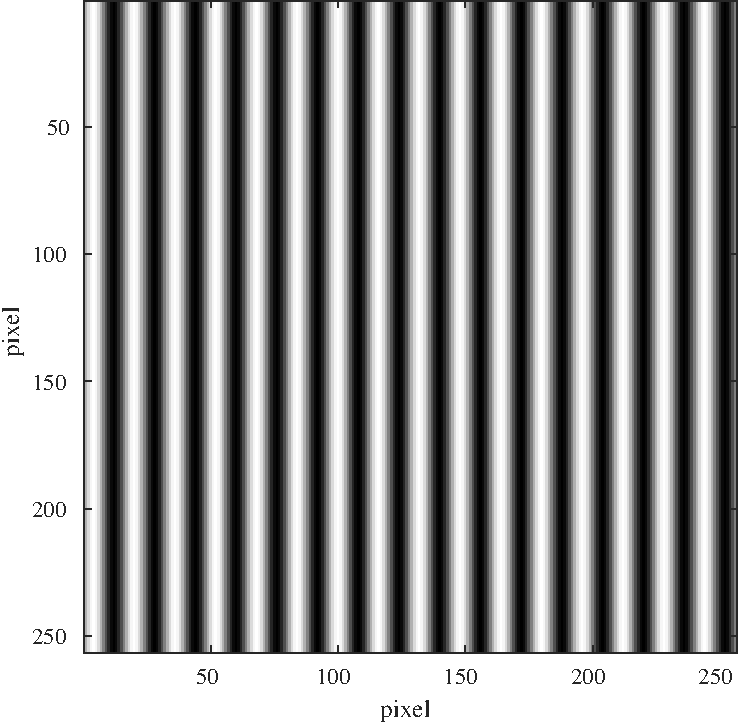
\includegraphics[width=\textwidth,keepaspectratio]{../../Figures/08_12_img16.pdf}
        \end{minipage} &
        \begin{minipage}{.25\textwidth}
            \centering
            \includegraphics[width=\textwidth,keepaspectratio]{../../Figures/08_13_img64.pdf}
        \end{minipage}                                  \\
        \vspace{.5em}                                                                                                     \\
        \begin{minipage}{.05\textwidth}
            \centering
            \rotatebox{90}{\small 縦縞\ パワースペクトル}
        \end{minipage}                                               &
        \begin{minipage}{.25\textwidth}
            \centering
            \axisfig{../../Figures/08_14_img4-fft.pdf}
        \end{minipage}                                        &
        \begin{minipage}{.25\textwidth}
            \axisfig{../../Figures/08_15_img16-fft.pdf}
        \end{minipage}                                       &
        \begin{minipage}{.25\textwidth}
            \axisfig{../../Figures/08_16_img64-fft.pdf}
        \end{minipage}                                                                        \\
        \vspace{.5em}                                                                                                     \\
        \begin{minipage}{.05\textwidth}
            \centering
            \rotatebox{90}{横縞}
        \end{minipage}                                                   &
        \begin{minipage}{.25\textwidth}
            \includegraphics[width=\textwidth,keepaspectratio]{../../Figures/08_21_img4.pdf}
        \end{minipage}  &
        \begin{minipage}{.25\textwidth}
            \includegraphics[width=\textwidth,keepaspectratio]{../../Figures/08_22_img16.pdf}
        \end{minipage} &
        \begin{minipage}{.25\textwidth}
            \includegraphics[width=\textwidth,keepaspectratio]{../../Figures/08_23_img64.pdf}
        \end{minipage}                                  \\
        \vspace{.5em}                                                                                                     \\
        \begin{minipage}{.05\textwidth}
            \centering
            \rotatebox{90}{\small 横縞\ パワースペクトル}
        \end{minipage}                                               &
        \begin{minipage}{.25\textwidth}
            \axisfig{../../Figures/08_24_img4-fft.pdf}
        \end{minipage}                                        &
        \begin{minipage}{.25\textwidth}
            \axisfig{../../Figures/08_25_img16-fft.pdf}
        \end{minipage}                                       &
        \begin{minipage}{.25\textwidth}
            \axisfig{../../Figures/08_26_img64-fft.pdf}
        \end{minipage}                                                                        \\
        \vspace{.5em}                                                                                                     \\
        \hline
    \end{tabularx}
    \caption{縦縞・横縞に対するフーリエ変換}
    \nextfloat
    \vspace{.5em}
    \begin{minipage}[b]{.15\textwidth}
        \centering
        \includegraphics[keepaspectratio,width=\textwidth]{../../LENNA.jpeg}
        \subcaption{元画像}
    \end{minipage}
    \begin{minipage}[b]{.15\textwidth}
        \centering
        \includegraphics[keepaspectratio,width=\textwidth]{../../Figures/08_41_filter.pdf}
        \subcaption{円形フィルタ\footnotemark[1]}
    \end{minipage}
    \begin{minipage}[b]{.15\textwidth}
        \centering
        \scalebox{.85}{\axisfig{../../Figures/08_42_fft.pdf}}
        \subcaption{\scriptsize パワースペクトル}
    \end{minipage}
    \begin{minipage}[b]{.15\textwidth}
        \centering
        \scalebox{.85}{\axisfig{../../Figures/08_43_fft-filter.pdf}}
        \subcaption{フィルタの適用\footnotemark[1]}
    \end{minipage}
    \begin{minipage}[b]{.15\textwidth}
        \centering
        \includegraphics[keepaspectratio,width=\textwidth]{../../Figures/08_44_fft-filter-50.pdf}
        \subcaption{\scriptsize フィルタ適用後\((50)\)}
    \end{minipage}
    \begin{minipage}[b]{.15\textwidth}
        \centering
        \includegraphics[keepaspectratio,width=\textwidth]{../../Figures/08_45_fft-filter-100.pdf}
        \subcaption{\scriptsize フィルタ適用後\((100)\)}
    \end{minipage}
    \caption{高域通過フィルタ}
\end{figure}
\footnotetext[1]{例として,半径が\(50\textrm{pixel}\)のフィルタを示す.}
\section{\consideration}
\paragraph{\kadaiaa}
実験結果より,原画像に近い画像は,緑チャネルだけを抜き出してグレイスケール画像として表示したものである.
また,赤チャネルと青チャネルを入れ替えた画像では,文字や建物の概形を,はっきりとらえることができる.
これらは,\eqref{equ:grayscale}でGreenの割合が一番多い理由と考えられる.
\paragraph{量子化数変換・階調変換・閾値処理}
量子化数を減らすことで,等高線のようなものが見える.
これは,元画像でなだらかな画素値の変化箇所が,量子化数を減らすことでとびとびの値になることで生じる.これを擬似輪郭という.
擬似輪郭は,量子化数を減らすことでより顕著になる.
量子化数が減ると擬似輪郭が生じる.この擬似輪郭は,階調反転しても変わらない.
さらに,閾値を調節することで,擬似輪郭を境に白と黒に別れることがわかった.
\paragraph{Sobelフィルタ,メディアンフィルタ}
メディアンフィルタは,ノイズに強いことがわかる.これは中央値を算出することにより,ノイズでない値が中央値となるからである.
ただし,画素値の中央値を抽出するため,平均値を算出する平滑化フィルタに比べて,計算量が多い.
それに対して,平滑化フィルタは,ノイズの画素値を含めた値の平均を算出するので,メディアンフィルタに比べるとノイズに弱い.
\paragraph{Sobelフィルタ,Laplacianフィルタ}
Sobelフィルタは,画像の隣接画素間の差分を計算する.よって,差が激しい画素の画素値が大きくなり,白く表示される.
つまり,ノイズに対してもエッジが強調される.
Laplacianフィルタは,画像の二次微分を計算することでエッジの位置を抽出している.Laplacianフィルタは高周波成分を増幅するため,ノイズに対してもエッジが強調される.
\paragraph{背景差分画像・色空間変換}
背景差分画像では,被写体がぼんやりと写っている.この画像に対して閾値処理することで,被写体を強調できることが分かった.
今回の実験では,閾値を手探りで探したため,実験結果の閾値が最適か分からない.
また,実験結果より,強調された部分は,光の当たり方や影の変化で白く光る部分もある.
ゆえに,背景差分画像だけでは,被写体の輪郭を正確にとらえることができないと考えられる.
HSV色空間では,この問題を解決できる.
RGB色空間では,明暗(影や光の状況)でRGB値が変わるのに対して,HSV色空間では,明暗が「明度」というチャネルで保存されているので,光の状況や影に左右されず,肌色領域をより正確に抽出できる.

\chapter{関連語句}
\section{ガボールフィルタ}
ガボールフィルタとは,画像を周波数領域でテクスチャ解析する方法のひとつ.
テクスチャ解析とは,粗い,滑らか,でこぼこなどの直感的な材質を,画素強度の空間的な変動の関数として定量化する試み\cite{テクスチャ解析}.
テクスチャ解析する方法として,フーリエ変換がある.フーリエ変換では画像をいくつかのブロックに区切る必要があり,対象の境界も同時に検出するという問題に対して,結果が粗くなる.
周波数の不正確さと,位置の不正確さとの積には下限があり,それを最小にするのは「ガボール関数」である.\par
ガボール関数は,サルの一次視覚野にある単純細胞の受容野特性によく似ており,ガボール関数の正弦波や余弦波の傾きを変化させることで.この受容野特性をよく再現できる.
\begin{flushright}
    \cite[p.144]{認知心理学辞典}
\end{flushright}
\section{固有顔法}
固有顔(eigenface)とは,顔画像の認識において最も有名な手法のひとつ.
顔認識では,顔を構成する部品(目や鼻,口など)の形状や,配置から特徴点を抽出して認識に利用する.しかし,照明方向や,撮影距離,表情,顔の傾きなどで顔の見え方が変わる.これらを許容したうえで正しく顔認識するには,顔画像をパターンとして扱い,統計的パターン認識手法を適用する方法がある.
まず挙げられるのが,パターン間のマッチングを用いた方法である.この方法は最も簡単なパターン認識手法であるが,画像そのものをパターンとして扱った場合,パターンの次元が大きくなる.
この問題を解決する方法として提案されたのが,固有顔である.固有顔は主成分分析によりパターンを情報圧縮し,顔画像の識別に利用している.
数枚の画像に対して,各画像から平均ベクトルを引いた集合に対して,固有値を求める.この時の固有ベクトルを固有顔と呼ぶ.\par
\hfill\cite{顔画像からの個人識別}
\section{オプティカルフロー}
視覚におけるオプティカルフローとは,前方へ移動する時の,後ろへ流れる背景のことである.
このオプティカルフローには2種類の特性があり,身体が対象に直線的な移動時に起きる「放射状オプティカルフロー」,身体が回るときに起きる「回転性のオプティカルフロー」が存在する\cite[p.679]{人間の運動学}.\par
また,動画像処理におけるオプティカルフローとは,動画像中の物体の動きを検出して,速度をべクトルで表示する手法を指す.
フロー推定方法としてブロックマッチング法を取り上げる.ブロックマッチング法は,画像のある大きさのブロックで分割し,次フレームにおける注目ブロックとの類似度が最も大きいブロックを検出する手法である\cite{オプティカルフローを用いた画像中の野鳥検出}.
\section{ストラクチャ フロム モーション(SfM: Structure from Motion)}
SfM\footnote{以後,ストラクチャ フロム モーションをSfMと記す.}とは,一連の2次元イメージから,3次元シーンの構造を推定するプロセスを指す\cite{SfM}.
具体的には,ドローンによる空撮写真(2次元)から3次元のデータを得るときに用いられる.

\bibliography{bib}
\chapter*{付録}
\addcontentsline{toc}{chapter}{付録}
\setcounter{section}{0}
\renewcommand{\thelstlisting}{src.\thesection-\arabic{lstlisting}}
\renewcommand{\thesection}{\Alph{section}}
\section{課題1}
\lstinputlisting[caption={01-01: \kadaiaa},label={src:01_01}]{../../01_EngineeringCharacteristicsOfSound/no1.m}
\lstinputlisting[caption={01-02: \kadaiab},label={src:01_02}]{../../01_EngineeringCharacteristicsOfSound/no2.m}
\end{document}